\section{Further Work}
\vspace{-2mm}
Whilst the system produced can be considered a complete system, there are still definitely improvements that could be made, and functionality that could be added. In this section, the main extensions to the system have been detailed, along with their reasoning for not being in the initial release. 

\subsection{Back end Interoperability}
\vspace{-2mm}
\label{sec:bei}
The purpose of the system is to be a web based front end, to a back end that can perform fuzzy inference. This means that the system should not be reliant on the back end that it currently uses (R-Shiny/FuzzyToolkitUoN), and it could be interchanged with some other back end (potentially with greater functionality, or better performance). This is a result of the system being written almost entirely in JavaScript, making the majority of it's functionality a client-sided affair, and not relying on the back end. The only functionality that the back end truly provides, is the ability to save files to the user's machine, and to evaluate the fuzzy system created. This means that, with the implementation of a simple API layer between the front end and back end, the back end could easily be swapped out to any back end that the user would want. This would allow the user extra functionality within the system, making it much more useful for the expert user. This could include such things as different inference types (like TSK), different t-norms, and t-conorms for the inference methods, and different visualisation techniques. This would make the system much more useful, as it currently can only perform Mamdani inference, with a limited number of inference methods, due to the limited scope of the back end. The revised architecture of the system, taking these interchangeable back ends into account, can be seen in figure \ref{fig:fw-interop}.

\begin{figure}[ht!]
	\begin{center}
		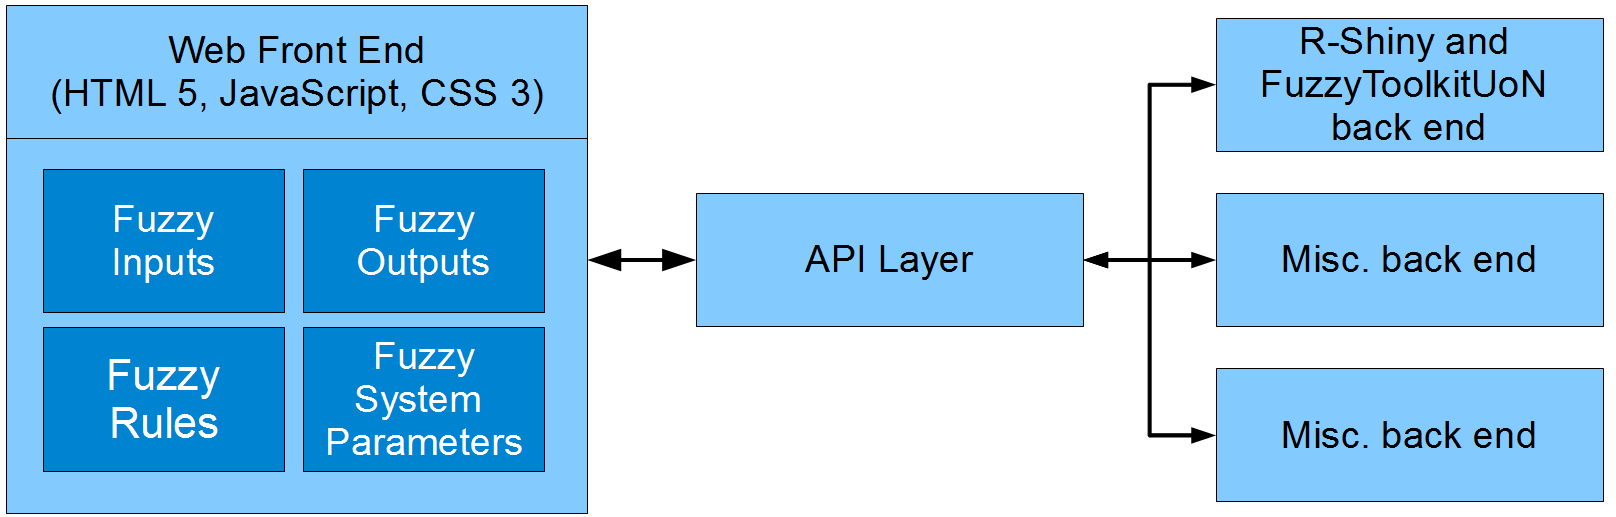
\includegraphics[width=0.8125\textwidth]{images/archi-new}
	\end{center}
	\vspace{-4mm}
	\caption{Interaction between the front end of the system and interchangeable back ends}
	\label{fig:fw-interop}
	\vspace{-3mm}
\end{figure}

\subsection{More Usability Improvements}
\vspace{-2mm}
\label{sec:mui}
As a result of the user evaluation that was detailed in section \ref{sec:uft}, many potential improvements to the system were identified. Most of these were personal preferences mentioned by few participants, but others were mentioned by more participants, and some thought should go into these features, if any more work is to be completed on the system.\ \\
\ \\
The first of these, noted by a handful of the participants with a high level of skill with computers, was the inability to press the return key, to save a membership function that had been created. Instead, the user was forced to click the ``Save Changes'' button. This was not a problem for the participants with a low level of skill with computers, as they generally use the mouse to navigate between input boxes. The expert users, however, were much more likely to use the tab key to navigate between the text boxes, and as a result, many of them expected that pressing the return key would save the membership function for them, so that they weren't required to use the mouse. This functionality \emph{is} available, but requires the user to press the tab key twice more after their final parameter, and then press the space bar; a combination that was not noticed or used, by many users. \ \\
\ \\
This leads onto the next possible improvement, of allowing more keyboard short cuts throughout the system. A good interface should be easy for novices to learn (which the results of the user feedback clearly indicate is true for this system), and efficient for experts to use. It has been found that, whilst most users do not use keyboard short cuts, they greatly increase the speed and efficient that tasks can be performed within a software system \cite{lane2005hidden}. Currently, the user is required to use the mouse for the majority of the system, which is much slower than a keyboard could be, once the user had mastered the keyboard short cuts.\ \\
\ \\
Another improvement that could be made, which would be useful for those wishing to learn how fuzzy logic works and for debugging purposes, would be the implementation of more visualisations of the inference process. Fuzzy inference is very easily representable graphically, and a display of these graphs on the evaluation page would be a great way for the user to learn how the inference process works so they could tweak their system accordingly, and gain a better understand of fuzzy logic as a whole. A mock up of how this could look is displayed in figure \ref{fig:fw-inf}.

\begin{figure}[ht!]
	\begin{center}
		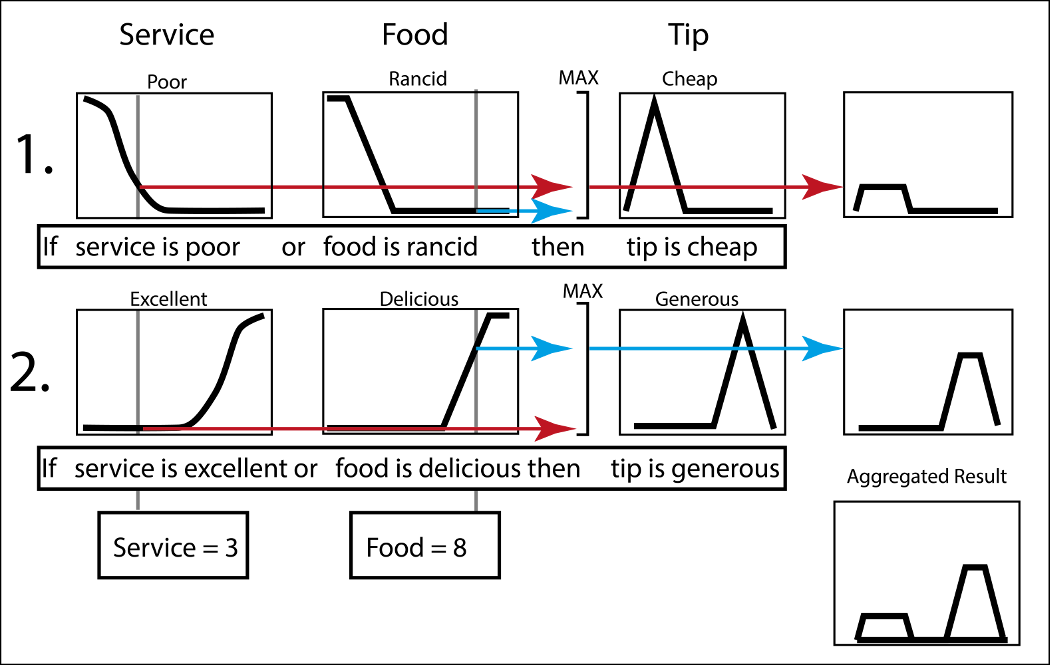
\includegraphics[width=0.9\textwidth]{images/inference}
	\end{center}
	\vspace{-2mm}
	\caption{Example of a possible way to display the fuzzy inference process}
	\label{fig:fw-inf}
	\vspace{-1mm}
\end{figure}

\noindent
The final improvement that could be made, would be the adoption of cookies within the system. Whilst this would present some security issues for the user, and would require a cookie agreement policy to be instated into the system, the addition of cookies could greatly increase user experience. The most obvious use of cookies would be the ability to auto-save the system the user is working on. This would mean that if they lost internet connection, or they accidentally closed the system, their work would not be lost, and they could continue working after restoring their work from a cookie. 
\newpage 
\subsection{Type-2 Fuzzy Logic Support}
\label{sec:type2}
The purpose of a type-1 fuzzy logic system, is to model uncertainty in the terms that humans use to describe properties. Unfortunately, this is slightly hypocritical; fuzzy sets have a connotation of uncertainty, but the membership functions used are entirely certain once their parameters have been specified \cite{mendel2003type}. Type-2 fuzzy logic attempts to rectify this, in the sense that uncertainty is not only limited to the terms used, but also the membership functions defined \cite{castillo2003type}. This means that each membership function defined has a third dimension, which allows an additional degree of freedom, to directly model uncertainty \cite{mendel2002type}. An example type-2 fuzzy set can be seen in figure \ref{fig:fw-type2}.
\begin{figure}[ht!]
	\begin{center}
		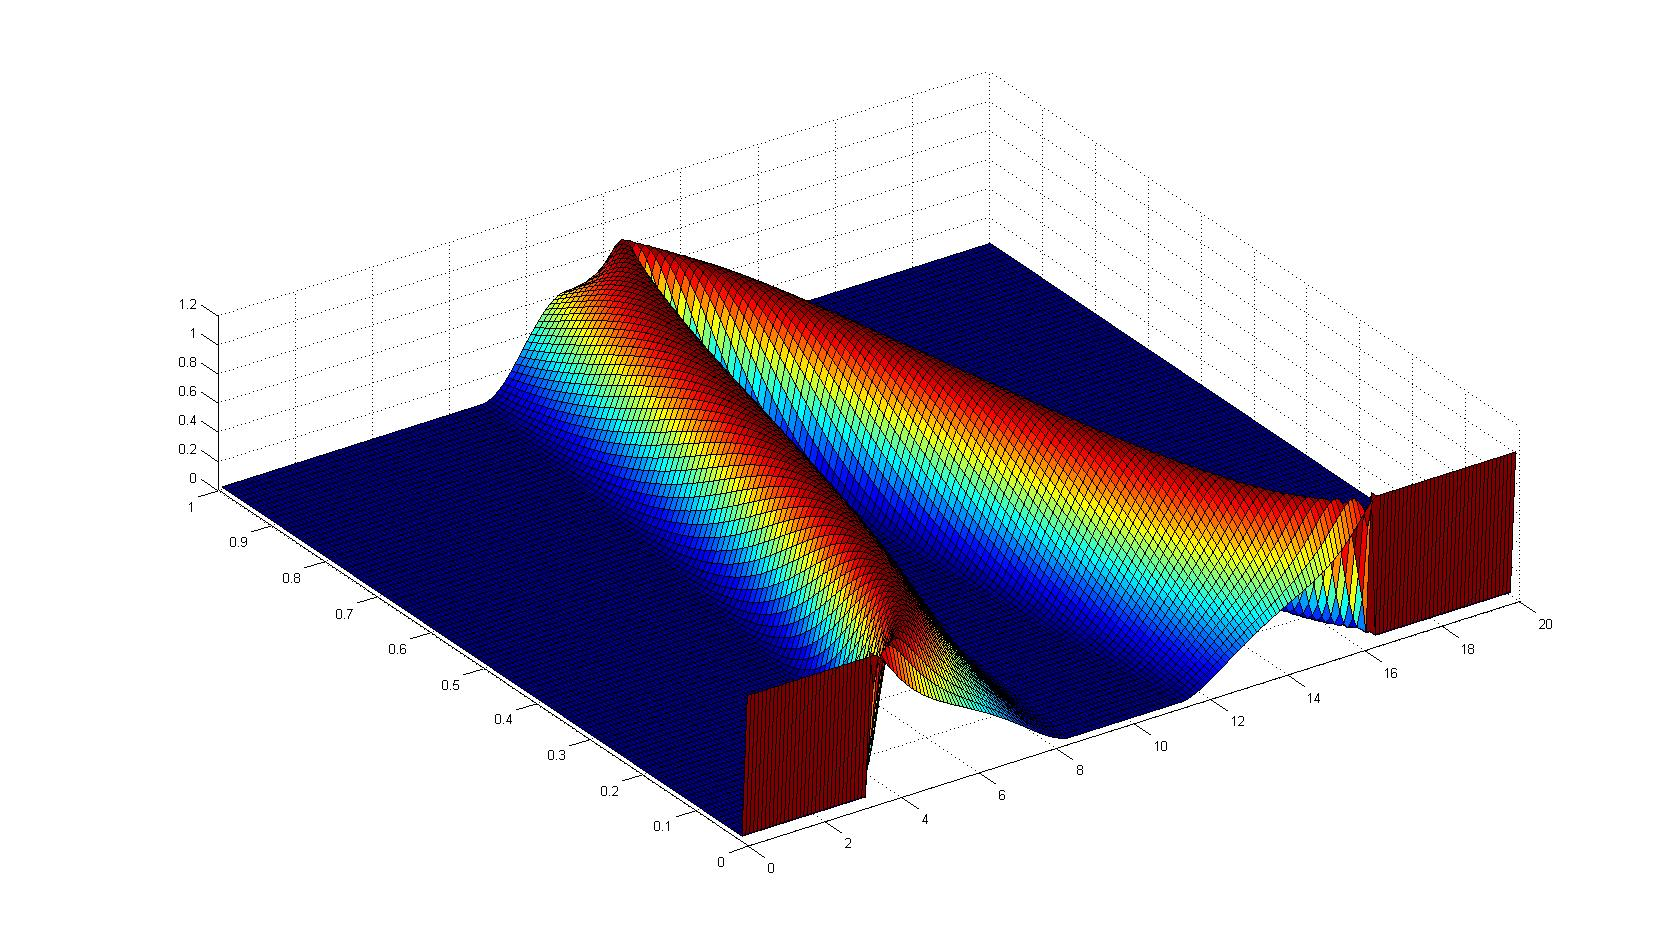
\includegraphics[width=0.5\textwidth]{images/type2set}
	\end{center}
	\vspace{-4mm}
	\caption{An example type-2 fuzzy set}
	\label{fig:fw-type2}
	\vspace{-1mm}
\end{figure}
\noindent
As mentioned in the introduction to this report, type-2 fuzzy logic is not supported in this software. This is because the jump in knowledge between type-1 fuzzy logic (that \emph{is} supported), and type-2, is extremely large, and would not be suitable for novice users. Other reasons include a lack of time to implement such a large feature, and that type-2 fuzzy logic is still not widely adopted in the field. If more time was allocated to the project, this could have been implemented alongside the type-1 system, however an entirely new back end would have been needed, as the current back end, FuzzyToolkitUoN, does not support type-2 fuzzy logic. Adding type-2 support to the system would have greatly improved it's usefulness and practicality, and could have easily made the tool a niche within the market, and the preferred software to use among experts. This would have been due to the ease of access, and ease of use of the system, which are  features that most type-2 software systems currently available are lacking (such as Juzzy \cite{wagner2013juzzy}, which requires an installation of Java before it can be used).

\subsection{Customisations}
The ability to customise a website has been identified as one of the key factors for website success \cite{fan2010factors}. It has been found that users are more likely to return to a piece of software, if it is customised to their needs, and thus more personal. Whilst there is not a huge number of customisations that could be made with a system like this, there are still some, and these could potentially stand to increase usability. One of these could be the look and feel of the system, which is currently a minimalistic white design. Some users prefer to use a darker interface (especially when completing work in the evening), and thus a set of different colour schemes could be employed, which would both serve a practical purpose, and an aesthetic one. Another potential customisation could be the ability to switch to an ``expert'' mode, where help is less present in the system, more keyboard short cuts are supported, and there is less GUI to navigate. This would greatly increase the speed in which an expert user could complete their task within the system, as there would be less distractions.